\chapter{Om Kojo}
\begin{multicols}{2}
\section*{\color{black}Vad är Kojo?}
Kojo är en app som hjälper dig att lära dig att programmera. Med Kojo kan du koda i det moderna och kraftfulla programspråket {\bf\color{blue}Scala}. Kojo är gratis och finns på Svenska. Kojo fungerar med Linux, Windows och Mac OSX.
\section*{\color{black}Var hittar jag Kojo?}
Ladda ner Kojo här: 
\\

\href{http://www.kogics.net/kojo-download}{www.kogics.net/kojo-download}
\\

Läs mer här: 
\\

\href{http://lth.se/programmera}{lth.se/programmera}

\columnbreak

\begin{center}
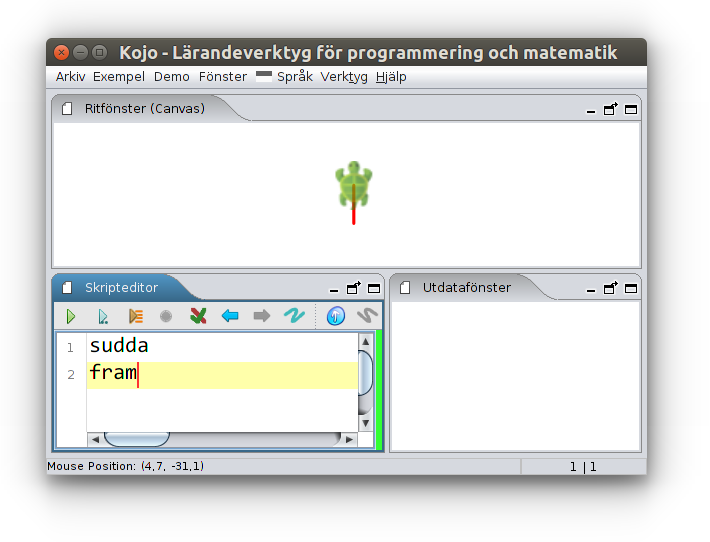
\includegraphics[width=14.0cm]{../img/kojo.png}
\end{center}

\end{multicols}

\chapter{Ditt första program}
\begin{multicols}{2}
\section*{\color{BrickRed}Uppdrag:}
Skriv så här i Kojos skripteditor-fönster:

\begin{lstlisting}[basicstyle={\ttfamily\fontsize{48}{58}\selectfont},numbers=none]
sudda
fram
\end{lstlisting}
        
Tryck på den gröna play-knappen 

\includegraphics[width=1.0cm]{../img/play.png}
\\

för att köra igång ditt program.

\columnbreak

\begin{center}
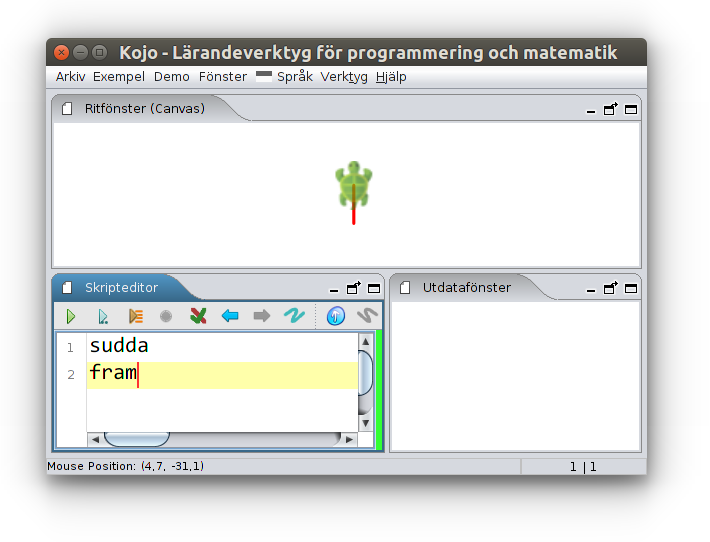
\includegraphics[width=14.0cm]{../img/fram.png}
\end{center}

\end{multicols}

\chapter{Rita en kvadrat}
\begin{multicols}{2}

\begin{lstlisting}[basicstyle={\ttfamily\fontsize{36}{43}\selectfont},numbers=none]
sudda
fram
höger
\end{lstlisting}
        
Om du skriver \lstinline{vänster} eller \lstinline{höger} så vrider sig paddan.
\section*{\color{BrickRed}Uppdrag:}
Utöka programmet så att det blir en kvadrat.

\columnbreak

\begin{center}
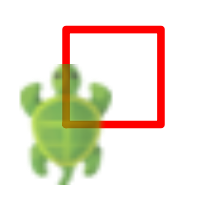
\includegraphics{../img/square.png}
\end{center}

\end{multicols}

\chapter{Rita en trappa}
\begin{multicols}{2}

\begin{lstlisting}[basicstyle={\ttfamily\fontsize{36}{43}\selectfont},numbers=none]
sudda
fram; vänster
fram; höger
\end{lstlisting}
        
\vskip 1.0em
Med semikolon \lstinline{;} kan du ha flera satser på samma rad.
\section*{\color{BrickRed}Uppdrag:}
Utöka programmet så att det blir en trappa.

\columnbreak

\begin{center}

\includegraphics{../img/stairs.png}
\end{center}

\end{multicols}

\chapter{Gör en loop}
\begin{multicols}{2}

\begin{lstlisting}[basicstyle={\ttfamily\fontsize{36}{43}\selectfont},numbers=none]
sudda
upprepa(4){ fram; höger }
\end{lstlisting}
        
\section*{\color{BrickRed}Uppdrag:}


\begin{itemize}

\item {Vad händer om du ändrar 4 till 100?}
\item {Rita en trappa med 100 trappsteg.}

\end{itemize}



\columnbreak

\begin{center}
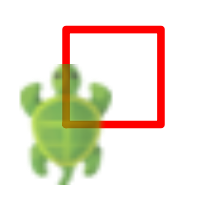
\includegraphics{../img/square.png}
\end{center}

\end{multicols}

\chapter{Rita en gubbe}
\begin{multicols}{2}
\section*{\color{BrickRed}Uppdrag:}
Rita en gubbe som du själv vill.
\section*{\color{OliveGreen}Tips:}

\begin{lstlisting}[basicstyle={\ttfamily\fontsize{20}{24}\selectfont},numbers=none]
hoppa
vänster(180)
fram(300)
hoppa(100)
hoppaTill(25,-28)
skriv("FELIX är bäst")
färg(lila)
fyll(grön)
\end{lstlisting}
        
Du kan se paddans läge nere till vänster medan du rör muspekaren i Ritfönstret:

\includegraphics[width=6.0cm]{../img/mousepos.png}


\columnbreak


\begin{center}
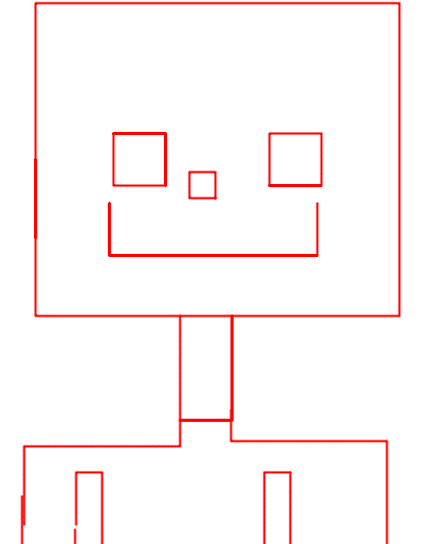
\includegraphics[width=4.5cm]{../img/man.png}
\end{center}

\vskip 2.0em
\begin{center}
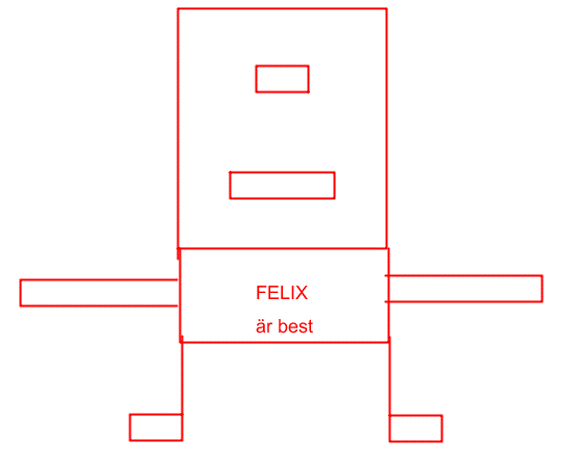
\includegraphics[width=9.0cm]{../img/alien.png}
\end{center}

\end{multicols}

\chapter{Hur snabb är din dator?}Den första elektroniska datorn hette {\bf ENIAC} och kunde räkna till 5000 på en sekund.\\
I Kojo finns en funktion \lstinline{räknaTill} som mäter hur snabbt datorn kan räkna.\\
När jag kör \lstinline{räknaTill(5000)} på min snabba dator skrivs detta i utdata-fönstret:

\begin{lstlisting}[numbers=none]

*** Räknar från 1 till ... 5000 *** KLAR!
Det tog 0.32 millisekunder.
      
\end{lstlisting}
        
\section*{\color{BrickRed}Uppdrag:}


\begin{itemize}

\item {Kör \lstinline{räknaTill(5000)} och kolla om din dator är snabbare än min.}
\item {Hur lång tid tar det för din dator att räkna till en miljon?}
\item {Hur långt hinner din dator räkna till på en sekund?}

\end{itemize}


\chapter{Spåra programmet}
\begin{multicols}{2}
\section*{\color{BrickRed}Uppdrag:}


\begin{itemize}

\item {Skriv ett program som ritar ett trappsteg.}
\item {Tryck på den brandgula play-knappen.}
\item {Klicka på ett av anropen: \lstinline{CALL fram}. Vad händer i Ritfönstret?}
\item {När en del av programmet är markerad med blått körs bara denna del om du trycker play. Avmarkera genom att klicka bredvid markeringen. }
\item {Lägg till fler satser i ditt program och se vad som händer när du spårar.}
\item {Stäng fönstret {\it Programspårning} när du är klar.}

\end{itemize}



\columnbreak

\begin{center}
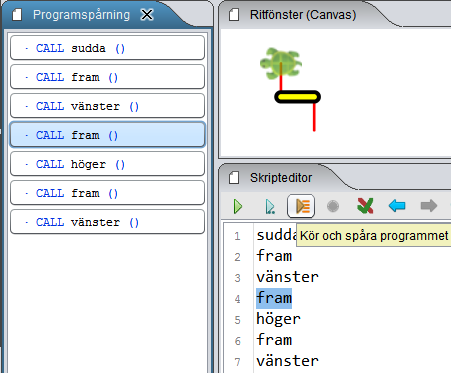
\includegraphics{../img/trace.png}
\end{center}

\end{multicols}

\chapter{Gör din egen funktion med \lstinline{def}}Med \lstinline{def} kan du göra egna {\it funktioner} som du själv väljer namn på.

\begin{lstlisting}[basicstyle={\ttfamily\fontsize{20}{24}\selectfont},numbers=none]
def kvadrat =  upprepa(4){ fram; höger }  

sudda
kvadrat    //använd din kvadrat-funktion
hoppa
kvadrat
\end{lstlisting}
        
\section*{\color{BrickRed}Uppdrag:}


\begin{itemize}

\item {Byt färg på kvadraterna.}
\item {Gör fler kvadrater.}

\end{itemize}


\section*{\color{OliveGreen}Tips:}

\begin{lstlisting}[numbers=none]
fyll(grön); färg(lila)
\end{lstlisting}
        
\chapter{Stapla kvadrater}
\begin{multicols}{2}
\section*{\color{BrickRed}Uppdrag:}
Gör en stapel med 10 kvadrater.
\section*{\color{OliveGreen}Tips:}
\vskip 1.0em

\begin{lstlisting}[numbers=none]
def kvadrat =  upprepa(4){ fram; höger }  

sudda; sakta(100)
upprepa(10){ ??? }
\end{lstlisting}
        

\columnbreak

\begin{center}
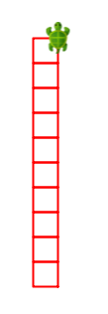
\includegraphics{../img/square-column.png}
\end{center}

\end{multicols}

\chapter{Gör en stapelfunktion}
\begin{multicols}{2}
\section*{\color{BrickRed}Uppdrag:}
Gör en funktion som heter \lstinline{stapel}, som ritar en stapel med 10 kvadrater.
\section*{\color{OliveGreen}Tips:}

\begin{lstlisting}[numbers=none]
def kvadrat = upprepa(4){ fram; höger }  
def stapel = ???

sudda; sakta(100)
stapel
\end{lstlisting}
        

\columnbreak

\begin{center}
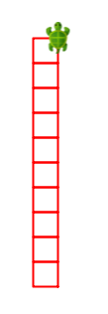
\includegraphics{../img/square-column.png}
\end{center}

\end{multicols}

\chapter{Gör ett rutnät}
\begin{multicols}{2}
\section*{\color{BrickRed}Uppdrag:}
Gör ett rutnät med 10*10 kvadrater.
\section*{\color{OliveGreen}Tips:}


\begin{itemize}

\item {Använd din stapelfunktion från tidigare.}
\item {Du kan hoppa baklänges en hel stapelhöjd med \lstinline{hoppa(-10*25)}}
\item {Du kan sedan hoppa till rätt plats med \lstinline{höger; hoppa; vänster}}

\end{itemize}



\columnbreak

\begin{center}
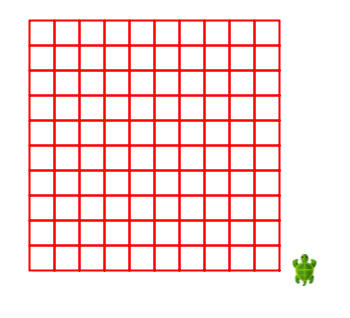
\includegraphics{../img/square-grid.png}
\end{center}

\end{multicols}

\chapter{Kvadrat med parameter}
\begin{multicols}{2}
\section*{\color{BrickRed}Uppdrag:}
Rita olika stora kvadrater.
\section*{\color{OliveGreen}Tips:}
Ge din kvadrat-funktion en {\it parameter},\\
med namnet \lstinline{sidlängd} och typen \lstinline{Heltal}:

\begin{lstlisting}[basicstyle={\ttfamily\fontsize{16}{19}\selectfont},numbers=none]
def kvadrat(sidlängd : Heltal) = 
  upprepa(4){ fram(sidlängd); höger }

sudda; sakta(100); osynlig
kvadrat(100) 
kvadrat(70)
kvadrat(40)
\end{lstlisting}
        
Du kan byta färg med:\\
\lstinline{fyll(blå); färg(rosa)}


\columnbreak


\begin{center}

\includegraphics[width=5.0cm]{../img/square-param.png}
\end{center}

\begin{center}
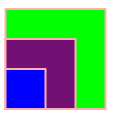
\includegraphics[width=5.0cm]{../img/square-param-color.png}
\end{center}

\end{multicols}

\chapter{Rita en kvadratgubbe}\section*{\color{BrickRed}Uppdrag:}
Rita en gubbe med hjälp av olika stora kvadrater.
\\


\begin{tikzpicture}[overlay]
\node at (20.0cm,0.5cm) {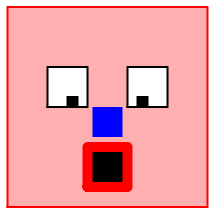
\includegraphics[width=5.5cm]{../img/square-man.png}};
\end{tikzpicture}
  
\section*{\color{OliveGreen}Tips:}

\begin{lstlisting}[basicstyle={\ttfamily\fontsize{14}{17}\selectfont},numbers=none]
def kvadrat(x: Heltal, y: Heltal, sidlängd: Heltal) = {
  hoppaTill(x, y)
  upprepa(4) { fram(sidlängd); höger }
}
def huvud(x: Heltal, y: Heltal) = { fyll(rosa); färg(röd); kvadrat(x, y, 200) }
def öga(x: Heltal, y: Heltal) = { fyll(vit); färg(svart); kvadrat(x, y, 40) }
def pupill(x: Heltal, y: Heltal) = { fyll(svart); färg(svart); kvadrat(x, y, 10) }
def näsa(x: Heltal, y: Heltal) = { fyll(blå); färg(genomskinlig); kvadrat(x, y, 30) }
def mun(x: Heltal, y: Heltal) = { bredd(10); fyll(svart); färg(röd); kvadrat(x, y, 40) }

sudda; sakta(20); osynlig
huvud(0, 0)
öga(40, 100); pupill(60, 100)
???
\end{lstlisting}
        
\chapter{Rita en polygon}\section*{\color{BrickRed}Uppdrag:}


\begin{itemize}

\item {Prova koden nedan. Rita olika slags polygoner.}
\item {Lägg till en parameter \lstinline{sidlängd} och rita olika stora polygoner.}
\item {Hur stort behöver n vara för att det ska se ut som en cirkel?}

\end{itemize}


\section*{\color{OliveGreen}Tips:}

\begin{lstlisting}[basicstyle={\ttfamily\fontsize{18}{22}\selectfont},numbers=none]
def polygon(n:Heltal) = upprepa(n){
  fram(100)
  vänster(360.0/n)
}

sudda; sakta(100)
polygon(7)
\end{lstlisting}
        

\begin{tikzpicture}[overlay]
\node at (20.0cm,3.5cm) {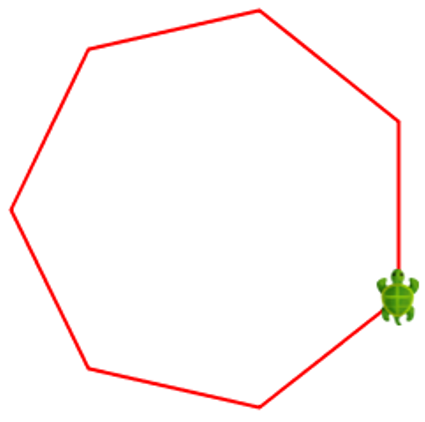
\includegraphics[width=8.0cm]{../img/polygon.png}};
\end{tikzpicture}
  
\chapter{Rita många polygoner}\section*{\color{BrickRed}Uppdrag:}


\begin{itemize}

\item {Prova programmet nedan.}
\item {Prova ändra antalet sidor och vinkel.}
\item {Fyll polygonerna med färg.}

\end{itemize}



\begin{tikzpicture}[overlay]
\node at (21.0cm,0.0cm) {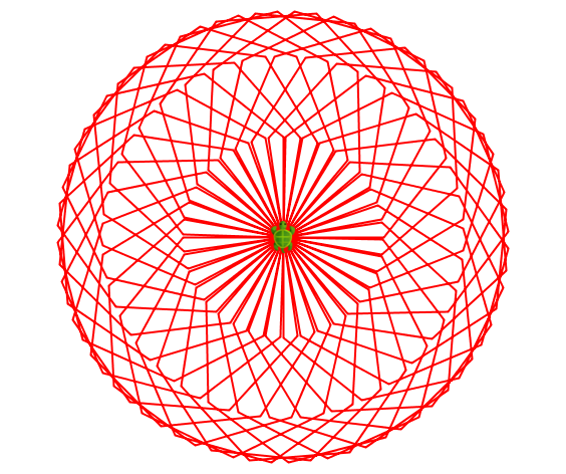
\includegraphics[width=12.0cm]{../img/polygons-circle.png}};
\end{tikzpicture}
  

\begin{lstlisting}[basicstyle={\ttfamily\fontsize{16}{19}\selectfont},numbers=none]
def polygon(n: Heltal, sidlängd: Heltal) = upprepa(n){
  fram(sidlängd)
  vänster(360.0/n)
}
def snurra(n: Heltal, vinkel: Heltal, sidlängd: Heltal) = 
  upprepa(360/vinkel){ polygon(n, sidlängd); vänster(vinkel) }

sudda; sakta(5)
snurra(7, 10, 100)
\end{lstlisting}
        
\chapter{Värden och uttryck}
\begin{multicols}{2}
\section*{\color{BrickRed}Uppdrag:}


\begin{itemize}

\item {Skriv \lstinline{1 + 1} och tryck på den blå play-knappen. Då skapar kojo en grön kommentar.}
\item {Kommentaren visar att värdet av uttrycket \lstinline{1 + 1} är \lstinline{2} och att typen är \lstinline{Int}, som betyder \lstinline{Heltal}.}
\item {Gör fler uträkningar. Vad det blir för värde och typ?}

\end{itemize}



\begin{lstlisting}[numbers=none]
5 * 5
10 + 2 * 5
"hej" + "på" + "dej"
5 / 2
5 / 2.0
5 % 2
\end{lstlisting}
        


\columnbreak


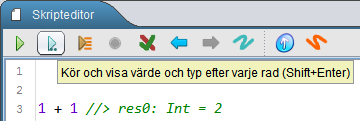
\includegraphics[width=12.0cm]{../img/show-value.png}
\section*{\color{OliveGreen}Tips:}


\begin{itemize}

\item {Med \lstinline{/} mellan heltal blir det heltalsdivision och decimalerna kastas bort. För att det ska bli division med decimaler måste minst ett av talen vara ett decimaltal.}
\item {Med \lstinline{%} får du resten vid en heltalsdivision.}

\end{itemize}


\end{multicols}

\chapter{Sätt namn på värden med \lstinline{val}}
\begin{multicols}{2}
\section*{\color{BrickRed}Uppdrag:}
Med \lstinline{val} kan du koppla ett namn till ett värde. Namnet kan sedan användas istället för värdet. Prova programmet nedan. Vad skriver paddan?

\begin{lstlisting}[numbers=none]
val x = 10
val y = 5
val gurka = x + y
val banan = x * y

sudda
fram; skriv(banan)
fram; skriv(gurka)
fram; skriv(y)
fram; skriv(x)
\end{lstlisting}
        

\columnbreak

\begin{center}
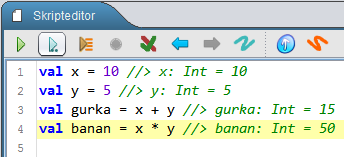
\includegraphics[width=12.0cm]{../img/val.png}
\end{center}

\end{multicols}

\chapter{Slumptal}\section*{\color{BrickRed}Uppdrag:}


\begin{itemize}

\item {Kör programmet nedan många gånger. Vad händer?}
\item {Vilket är det minsta och största möjliga värdet på radien \lstinline{r}?}
\item {Ändra så att \lstinline{r} blir ett slumptal mellan 3 och 200.}
\item {Rita 100 cirklar med slumpmässig radie på slumpmässig plats, som bilden visar.}

\end{itemize}



\begin{tikzpicture}[overlay]
\node at (21.0cm,-5.0cm) {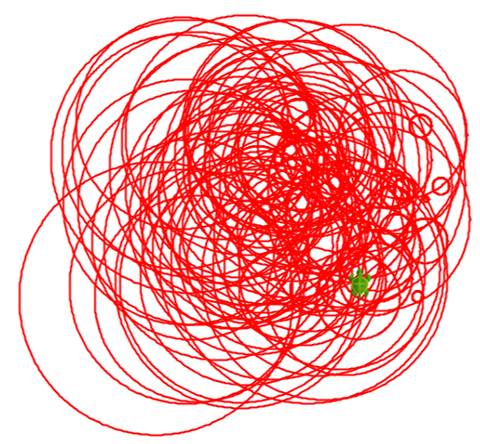
\includegraphics[width=8.0cm]{../img/random-circles.png}};
\end{tikzpicture}
  

\begin{lstlisting}[basicstyle={\ttfamily\fontsize{20}{24}\selectfont},numbers=none]
//värdet r blir ett slumptal mellan 10 och 89:
val r = slumptal(90) + 10   

sudda; sakta(10); osynlig
skriv("Radie = " + r)
cirkel(r)
\end{lstlisting}
        
\chapter{Blanda dina egna färger}

\begin{itemize}

\item {Med \lstinline{Color} kan du blanda egna färger, till exempel \lstinline{Color(0, 70, 0)}}
\item {De tre parametrarna anger mängden {\it rött}, {\it grönt} och {\it blått}}
\item {Du kan också lägga till en fjärde parameter som anger {\it genomskinligheten}}
\item {Alla parametrar ska vara mellan 0 och 255}

\end{itemize}


\section*{\color{BrickRed}Uppdrag:}
Prova programmet nedan. Ändra genomskinligheten.

\begin{tikzpicture}[overlay]
\node at (23.0cm,-2.0cm) {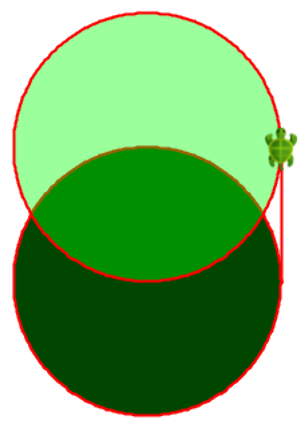
\includegraphics[width=7.0cm]{../img/color-circles.png}};
\end{tikzpicture}
  

\begin{lstlisting}[basicstyle={\ttfamily\fontsize{16}{19}\selectfont},numbers=none]
sudda; sakta(100)      

val olivgrön = Color(0,70,0)
val pistageglass = Color(0,255,0,100)

fyll(olivgrön); cirkel(100)
fyll(pistageglass); fram(100); cirkel(100)
\end{lstlisting}
        
\chapter{Prova färgväljaren}
\begin{multicols}{2}
\section*{\color{BrickRed}Uppdrag:}


\begin{itemize}

\item {Högerklicka i editor-fönstret och klicka på "Välj färg".}
\item {Om du väljer fliken {\bf RGB} i färgväljaren kan du blanda nya RGB-färger.}
\item {Tryck OK och titta i Utdatafönstret. Där syns de tre RGB-värdena för rött, grönt och blått.}
\item {Du kan använda dessa värden i ditt program för att rita med din nya färg med \lstinline{färg(Color(218, 153, 67))}.}

\end{itemize}



\columnbreak

\begin{center}
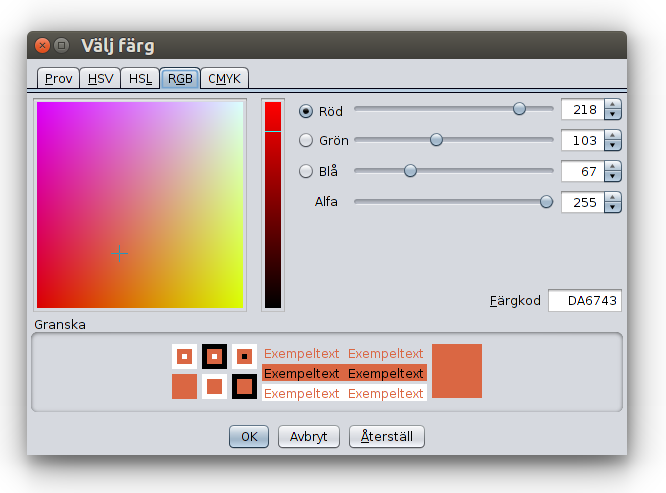
\includegraphics[width=14.0cm]{../img/color-chooser-rgb-sv.png}
\end{center}

\end{multicols}

\chapter{Rita slumpcirklar}
\begin{multicols}{2}

\begin{lstlisting}[basicstyle={\ttfamily\fontsize{16}{19}\selectfont},numbers=none]
def slump = slumptal(256)
def slumpfärg = Color(slump,10,slump,100) 

sudda; sakta(5)
bakgrund2(svart,vit)
bredd(6)

upprepa(100) {
    färg(slumpfärg)
    cirkel(100)
    hoppa(20)
    höger(35)
}
\end{lstlisting}
        
\section*{\color{BrickRed}Uppdrag:}
Prova olika slumpfärger och bakgrunder.


\columnbreak


\begin{center}
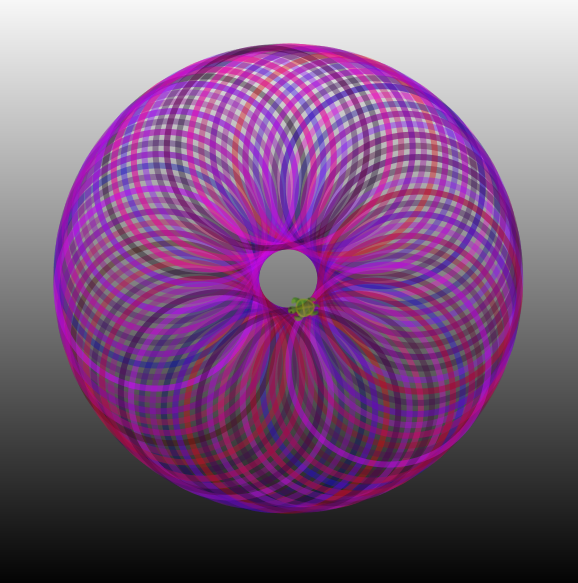
\includegraphics[width=12.0cm]{../img/circle-of-circles.png}
\end{center}

\end{multicols}

\chapter{Rita en blomma}\section*{\color{BrickRed}Uppdrag:}
Programmet nedan ritar 100 slumpfärgade cirklar på slumpmässig plats med slumpmässig radie. Prova att ändra de olika slumptalens gränser och försök förklara vad som händer.

\begin{tikzpicture}[overlay]
\node at (21.5cm,-4.0cm) {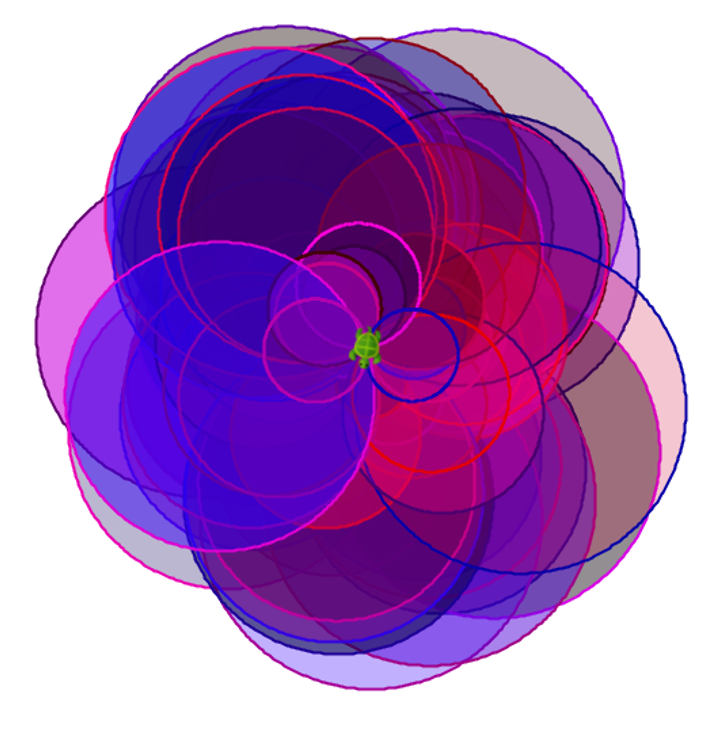
\includegraphics[width=9.0cm]{../img/random-color-circles.png}};
\end{tikzpicture}
  

\begin{lstlisting}[basicstyle={\ttfamily\fontsize{16}{19}\selectfont},numbers=none]
sudda(); sakta(5)
bredd(2)
upprepa(100){
  färg(Color(slumptal(256),0,slumptal(256)))
  fyll(Color(slumptal(256),0,slumptal(256),slumptal(100)+50))
  vänster(slumptal(360))
  cirkel(slumptal(30)*4+10)
}
\end{lstlisting}
        
\chapter{Skapa en variabel med \lstinline{var}}Med \lstinline{var} kan koppla ett namn till ett värde.\\
Du får då en variabel, som kan tilldelas ett nytt värde så här:

\begin{lstlisting}[numbers=none]

var gurka = 1
gurka = 1 + 1   //först räknas 1 + 1 ut, sedan blir gurka 2        
        
\end{lstlisting}
        
\section*{\color{BrickRed}Uppdrag:}
Prova programmet nedan. Vad skriver paddan?

\begin{lstlisting}[basicstyle={\ttfamily\fontsize{16}{19}\selectfont},numbers=none]
var i = 0

sudda
upprepa(10){
  i = i + 1
  fram; skriv(i)
}
\end{lstlisting}
        
\section*{\color{OliveGreen}Tips:}


\begin{itemize}

\item {I satsen \lstinline{i = i + 1} tilldelas \lstinline{i} ett nytt värde som blir det {\it gamla} värdet av \lstinline{i} plus \lstinline{1}}

\end{itemize}


\chapter{Rita många blommor}\section*{\color{BrickRed}Uppdrag:}


\begin{itemize}

\item {Gör en funktion som heter \lstinline{blomma}, som ritar en krona och en grön stjälk från kronans mitt med ett grönt blad.}
\item {Rita 5 blommor bredvid varandra.}

\end{itemize}



\begin{tikzpicture}[overlay]
\node at (15.0cm,-7.0cm) {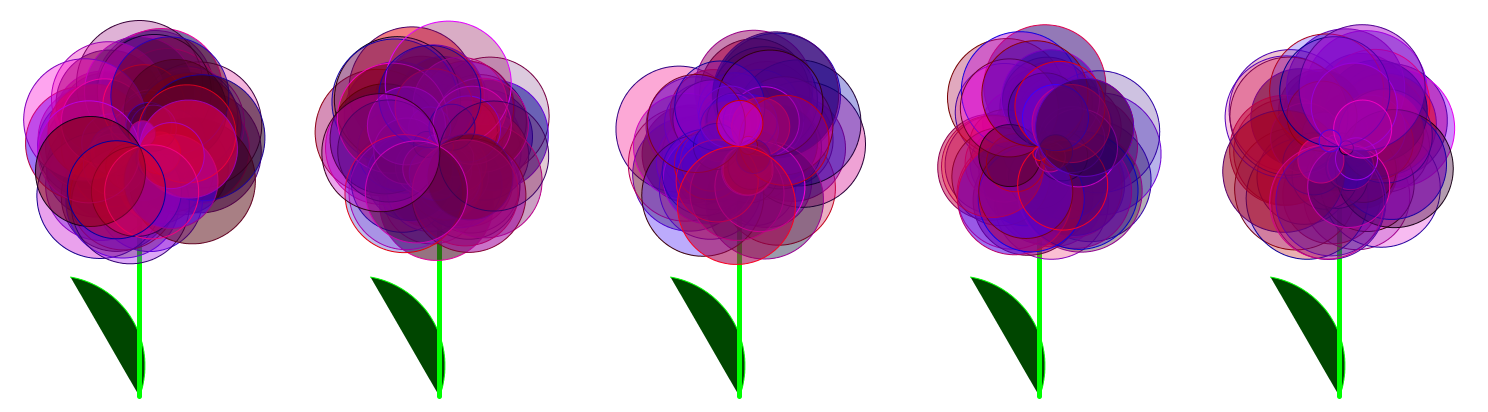
\includegraphics[width=16.0cm]{../img/flowers.png}};
\end{tikzpicture}
  
\section*{\color{OliveGreen}Tips:}
Du kan rita blad med \lstinline{båge(radie, vinkel)}. \\
Låt funktionen \lstinline{blomma} ha två parametrar x och y och använd \lstinline{hoppaTill(x,y)}\\
Du kan loopa 5 gånger och räkna ut platsen så här:

\begin{lstlisting}[basicstyle={\ttfamily\fontsize{18}{22}\selectfont},numbers=none]
var i = 0          
upprepa(5){
  blomma(600*i,0)
  i = i + 1        
}
\end{lstlisting}
        
\chapter{Byt kostym på paddan}\section*{\color{BrickRed}Uppdrag:}
Ladda ner mediafiler från Kojos hemsida:
\href{http://www.kogics.net/kojo-download#media}{www.kogics.net/kojo-download\#media}


\begin{itemize}

\item {Packa upp filen \lstinline{scratch-media.zip} och leta rätt på hästbilden \lstinline{horse1-a.png} i mappen \lstinline{Media/Costumes/Animals}}
\item {Lägg filen \lstinline{horse1-a.png} i samma mapp som du har ditt program.}
\item {Prova att byta kostym på paddan till en häst så här:}

\end{itemize}



\begin{tikzpicture}[overlay]
\node at (22.0cm,-2.5cm) {
\includegraphics{../img/horse1-a.png}};
\end{tikzpicture}
  

\begin{lstlisting}[basicstyle={\ttfamily\fontsize{20}{24}\selectfont},numbers=none]
sudda
kostym("horse1-a.png")  
sakta(2000)
fram(1000)
\end{lstlisting}
        
\section*{\color{OliveGreen}Tips:}


\begin{itemize}

\item {Du kan också använda dina egna bilder av typen \lstinline{.png} eller \lstinline{.jpg}}
\item {Om du vill lägga bilden i en annan mapp så kan du skriva filens sökväg, till exempel \lstinline{kostym("~/Kojo/Media/Costumes/Animals/horse1-a.png")} där \lstinline{~} betyder din hemkatalog.}

\end{itemize}


\chapter{Gör många paddor}
\chapter{Gissa talet}
\begin{lstlisting}[basicstyle={\ttfamily\fontsize{16}{19}\selectfont},numbers=none]
val hemlis = slumptal(100)+1
var svar = indata("Gissa ett tal mellan 1 och 100! ")
var fortsätt = true

while (fortsätt) {
    if (svar.toInt < hemlis)
      svar = indata(svar + " är för LITET, gissa igen!")
    else if (svar.toInt > hemlis)
      svar = indata(svar + " är för STORT, gissa igen!")
    else if (svar.toInt == hemlis)
      fortsätt = false
}
utdata(hemlis + " är RÄTT svar!")
\end{lstlisting}
        
\section*{\color{BrickRed}Uppdrag:}
Inför en variabel \lstinline{var antalFörsök = 0} och se till att utskriften på slutet blir:\\
\lstinline{Rätt svar! Du klarade det på 5 gissningar}
\chapter{Träna multiplikation}
\begin{lstlisting}[basicstyle={\ttfamily\fontsize{16}{19}\selectfont},numbers=none]
var antalRätt = 0
val startTid = System.currentTimeMillis / 1000
upprepa(12) {
  val tal1 = slumptal(12)+1
  val tal2 = slumptal(12)+1
  val svar = indata("Vad är " + tal1 + "*" + tal2 + "?")
  if (svar == (tal1 * tal2).toString) {
    utdata("Rätt!")
    antalRätt = antalRätt + 1
  }
  else utdata("Fel. Rätt svar är " + (tal1 * tal2))
}
val stoppTid = System.currentTimeMillis / 1000
val sek = stoppTid - startTid
utdata("Du fick " + antalRätt + " rätt på " + sek + " sekunder.")
\end{lstlisting}
        
\section*{\color{BrickRed}Uppdrag:}
Ändra så att man bara tränar 8:ans och 9:ans tabell.
\chapter{Spara djur i en vektor}
\begin{lstlisting}[basicstyle={\ttfamily\fontsize{16}{19}\selectfont},numbers=none]
var djur = Vector("älg", "ko", "kanin", "kvalster")  //variablen djur blir en vektor med 4 djur
utdata("Första djuret i vektorn är: " + djur(0))     //platserna i vektorer räknas från 0
utdata("Andra djuret i vektorn är:  " + djur(1))
utdata("Det finns så här många djur: " + djur.size)
utdata("Sista djuret i vektorn är:  " + djur(djur.size-1))

val s = slumptal(djur.size)   //dra ett slumpal mellan 0 och antalet djur minus 1
utdata("Ett slumpmässigt djur: " + djur(s))

djur = djur :+ "kamel"    //lägg till ett djur sist i vektorn
djur = "dromedar" +: djur //lägg till ett djur först i vektorn
djur = djur.updated(2, "slamkrypare")  //Ändra tredje djuret (plats 2 i vektorn)
utdata("Alla djur i vektorn baklänges:")
djur.foreach{x => utdata(x.reverse)} //för alla x i vektorn: skriv ut x baklänges
\end{lstlisting}
        
\section*{\color{BrickRed}Uppdrag:}


\begin{itemize}

\item {Vad skriver programmet i utdatafönstret? Förklara vad som händer.}
\item {Lägg till fler djur i vektorn.}

\end{itemize}


\chapter{Träna glosor}
\begin{lstlisting}[basicstyle={\ttfamily\fontsize{16}{19}\selectfont},numbers=none]
val svenska = Vector("dator", "sköldpadda", "cirkel")
val engelska = Vector("computer", "turtle", "circle")
var antalRätt = 0
upprepa(5) {
  val s = slumptal(3)
  val glosa = svenska(s)
  val svar = indata("Vad heter " + glosa + " på engelska?")
  if (svar == engelska(s)) {
    utdata("Rätt svar!")
    antalRätt = antalRätt + 1
  } else {
    utdata("Fel svar. Rätt svar är: " + engelska(s))
  }
}
utdata("Du fick" + antalRätt + " rätt.")
\end{lstlisting}
        
\section*{\color{BrickRed}Uppdrag:}


\begin{itemize}

\item {Lägg till fler glosor.}
\item {Träna på glosor från engelska till svenska.}
\item {Låt användaren välja hur många frågor innan avslut. Tips: \lstinline{val antal = indata("Ange antal: ").toInt}}

\end{itemize}


\chapter{Huvudstadsspelet}
\begin{lstlisting}[basicstyle={\ttfamily\fontsize{13}{16}\selectfont},numbers=none]
def huvudstadsspelet = {
  println("Välkommen till Huvudstadsspelet!")
  val stad = Map("Sverige" ->"Stockholm", "Danmark" -> "Köpenhamn", "Skåne" -> "Malmö")
  var länderKvar = stad.keySet //keySet ger en mängd av alla nycklar i en Map 
  def slumpLand = scala.util.Random.shuffle(länderKvar.toVector).head
  while(!länderKvar.isEmpty) {
    val land = slumpLand
    val svar = indata("Vad heter huvudstaden i " + land + "?")
    utdata(s"Du skrev: $svar")
    if (svar == stad(land)) {
      utdata("Rätt svar! Du har " + länderKvar.size + " länder kvar!")
      länderKvar = länderKvar - land  //ta bort land ur mängden länderKvar
    } else {
      utdata(s"Fel svar. Huvudstaden i $land börjar på ${stad(land).take(2)}...")
    }
  }
  utdata(s"TACK FÖR ATT DU KÄMPADE! (Tryck ESC)")
}

toggleFullScreenOutput;  
setOutputBackground(black);setOutputTextColor(green); setOutputTextFontSize(30)
upprepa(100)(utdata("")) //scrolla utdafönstret med 100 blanka rader

huvudstadsspelet

// *** UPPDRAG: (1) Lägg till fler par: land -> stad  (2) Mät tid och räkna poäng.
\end{lstlisting}
        
\chapter{Gör en timer}
\begin{lstlisting}[basicstyle={\ttfamily\fontsize{14}{17}\selectfont},numbers=none]
object timer {
  def nu = System.currentTimeMillis  //ger nutid i millisekunder
  var tid = nu
  def nollställ = { tid = nu }
  def mät = nu - tid
  def slumpvänta(min: Int, max: Int) =  //vänta mellan min och max sekunder
    Thread.sleep((slumptal(max-min)+min)*1000)  //Thread.sleep(1000) väntar 1 sekund
}

utdata("Klicka i utdatafönstret och vänta...")
timer.slumpvänta(3,6)   //vänta mellan 3 och 6 sekunder
timer.nollställ
indata("Tryck Enter så snabbt du kan.")
utdata("Reaktionstid: " + (timer.mät/1000.0) + " sekunder")
\end{lstlisting}
        
\section*{\color{BrickRed}Uppdrag:}


\begin{itemize}

\item {Prova programmet och mät din reaktionstid. Hur snabb är du?}
\item {Använd \lstinline{timer} i uppdraget {\it Gissa talet} och lägg till utskriften: \lstinline{Rätt svar! Du klarade det på 5 gissningar och 32 sekunder}}

\end{itemize}


\chapter{Simulera ett trafikljus}
\begin{tikzpicture}[overlay]
\node at (22.0cm,-6.0cm) {
\includegraphics[width=3.0cm]{../img/traffic-lights.png}};
\end{tikzpicture}
  

\begin{lstlisting}[basicstyle={\ttfamily\fontsize{14}{17}\selectfont},numbers=none]
def släckAlla = draw(penColor(gray) * fillColor(black) -> PicShape.rect(130,40))
def ljus(c: Color, h: Int) = penColor(noColor) * fillColor(c) * trans(20,h) -> PicShape.circle(15)
def tändRött = draw(ljus(red, 100))
def tändGult = draw(ljus(yellow, 65))
def tändGrönt = draw(ljus(green, 30))
def vänta(sekunder: Int) = Thread.sleep(sekunder*1000)

sudda; osynlig  
while (true) { //en oändlig loop
  släckAlla
  tändRött;  vänta(3)
  tändGult;  vänta(1) 
  släckAlla
  tändGrönt; vänta(3)
  tändGult;  vänta(1)
}
\end{lstlisting}
        
\section*{\color{BrickRed}Uppdrag:}


\begin{itemize}

\item {Hur växlar trafikljuset? Försök förklara vad som händer.}
\item {Ändra så att trafikljuset är grönt dubbelt så länge.}

\end{itemize}


\chapter{Styr paddan med tangentbordet}
\begin{multicols}{2}

\begin{lstlisting}[basicstyle={\ttfamily\fontsize{18}{22}\selectfont},numbers=none]
sudda; sakta(0)
activateCanvas()

animate { fram(1) }

onKeyPress { k =>
  k match {
    case Kc.VK_LEFT =>   vänster(5)
    case Kc.VK_RIGHT =>  höger(5)
    case Kc.VK_SPACE =>  fram(5)
    case _ => 
      utdata("Annan tangent: " + k)
  }
}
\end{lstlisting}
        


\columnbreak


\section*{\color{BrickRed}Uppdrag:}


\begin{itemize}

\item {Skriv \lstinline{Kc.} och tryck \lstinline{Ctrl+Alt+Mellanslag} och kolla vad de olika tangenterna heter.}
\item {Gör \lstinline{pennaUpp} om man trycker pil upp}
\item {Gör \lstinline{pennaNer} om man trycker pil ner}
\item {Gör \lstinline{färg(blå)} om man trycker B}
\item {Gör \lstinline{färg(röd)} om man trycker R}
\item {Öka eller minska hastigheten om man trycker + eller -}

\end{itemize}


\end{multicols}

\chapter{Styr paddan med musen}
\begin{multicols}{2}

\begin{lstlisting}[basicstyle={\ttfamily\fontsize{16}{19}\selectfont},numbers=none]
sudda; sakta(100)
activateCanvas()

var rita = true

onKeyPress { k =>
  k match {
    case Kc.VK_DOWN => 
      penDown()
      rita = true
    case Kc.VK_UP => 
      penUp()
      rita = false
    case _ => 
      utdata("Annan tangent: " + k)
  }
}

onMouseClick { (x, y) =>
  if (rita) moveTo(x, y) else jumpTo(x, y)
}
\end{lstlisting}
        


\columnbreak


\section*{\color{BrickRed}Uppdrag:}


\begin{itemize}

\item {Gör \lstinline{fyll(svart)} om man trycker på F}
\item {Inför en variabel \lstinline{var fyllNästa = true} och i fallet att man trycker på \lstinline{Kc.VK_F} gör:}

\end{itemize}



\begin{lstlisting}[numbers=none]

      if (fyllNästa) {
        fyll(svart)
        fyllNästa=false
      } else {
        fyll(genomskinlig)
        fyllNästa=true
      }
      
\end{lstlisting}
        
\end{multicols}

\chapter{Gör ett ditt eget bankkonto}
\begin{multicols}{2}

\begin{lstlisting}[basicstyle={\ttfamily\fontsize{16}{19}\selectfont},numbers=none]
object mittKonto {
  val nummer = 123456
  var saldo = 0.0
  def in(belopp: Decimaltal) = {
    saldo = saldo + belopp 
  }
  def ut(belopp: Decimaltal) = { 
    saldo = saldo - belopp 
  }
  def visaSaldo() = {
    utdata("Konto nummer: " + nummer) 
    utdata("       saldo: " + saldo)
  }
}

mittKonto.visaSaldo()
mittKonto.in(100)
mittKonto.visaSaldo()
mittKonto.ut(10)
mittKonto.visaSaldo()
\end{lstlisting}
        


\columnbreak


\section*{\color{BrickRed}Uppdrag:}


\begin{itemize}

\item {Vad är saldot efter att programmet kört klart? Förklara vad som händer.}
\item {Gör så att det inte går att ta ut mer pengar än som finns på kontot.}
\item {Lägg till \lstinline{val maxBelopp = 5000} och kolla så att man inte kan ta ut mer än \lstinline{maxBelopp} åt gången.}

\end{itemize}


\end{multicols}

\chapter{Gör många konto med en klass}
\begin{multicols}{2}
Om man vill skapa många konto behövs en klass. Med \lstinline{new} skapas nya objekt. Varje objekt får eget nummer och saldo.

\begin{lstlisting}[basicstyle={\ttfamily\fontsize{14}{17}\selectfont},numbers=none]
class Konto(nummer: Heltal) {
  var saldo = 0.0 
  def in(belopp: Decimaltal) = {
    saldo = saldo + belopp
  }
  def ut(belopp: Decimaltal) = {
    saldo = saldo - belopp
  }
  def visaSaldo() = 
    utdata(s"Konto $nummer: $saldo")
}

val konto1 = new Konto(12345) //new skapar objekt 
val konto2 = new Konto(67890) //ännu ett objekt

konto1.in(99)
konto2.in(88)
konto1.ut(57)
konto1.visaSaldo()
konto2.visaSaldo()
\end{lstlisting}
        


\columnbreak


\section*{\color{BrickRed}Uppdrag:}


\begin{itemize}

\item {Vad är saldot på de olika kontona när programmet kört klart? Förklara vad som händer.}
\item {Skapa ännu fler bankkonto-objekt och sätt in och ta ut lite pengar på dessa.}
\item {Lägg till en klassparameter \lstinline{namn: String} som ska innehålla namnet på kontoägaren när objekt skapas.}
\item {Gör så att även \lstinline{namn} skrivs ut när \lstinline{visaSaldo} anropas}

\end{itemize}


\end{multicols}

\chapter{Prata med datorn}
\begin{lstlisting}[basicstyle={\ttfamily\fontsize{13}{16}\selectfont},numbers=none]
setOutputBackground(black); setOutputTextFontSize(30); setOutputTextColor(green)
utdata("Skriv intressanta svar även om frågorna är konstiga. Avsluta med 'hej då'")
def slumpa(xs: Vector[String]) = scala.util.Random.shuffle(xs).head
val ledtexter = Vector("Vad betyder", "Gillar du", "Varför behövs", "Berätta mer om")
var svar = "?"
val öppning = "Vad vill du prata om?"
var ord = Vector("navelludd", "ketchupglass", "jultomten", "örngott") 
while (svar != "hej då") {
  val t = if (svar == "?") öppning 
    else if (svar == "nej") "Nähä." 
    else if(svar == "ja") "Jaha." 
    else if (svar.length < 4) "Jasså..." 
    else slumpa(ledtexter) + " " + slumpa(ord) + "?"
  svar = indata(t).toLowerCase
  ord = ord ++ svar.split(" ").toList.filter(_.length > 3) 
} 
utdata("Tack för pratstunden! Jag kan nu dessa ord:" + ord)

//Uppdrag:
// (1) Prova programmet och försök att förklara vad som händer.
// (2) När avslutas while-loopen?
// (3) Lägg till fler strängar i vektorerna ledtexter och ord
// (4) Lägg till fler bra svar på några korta ord utöver "nej" och "ja"
\end{lstlisting}
        
\chapter{Modda pong-spelet}
\begin{multicols}{2}
\section*{\color{BrickRed}Uppdrag:}


\begin{itemize}

\item {Välj menyn Exempel > Animeringar och spel > Pong och prova spelet.}
\item {Man styr med pil upp och pil ner, samt A och Z.}
\item {Tryck ESC för att avbryta spelet och undersök koden.}
\item {Ändra i koden så att bollen blir större.}
\item {Gör spelplanen till en tennisplan, med grönt underlag, vita linjer och en gul boll.}

\end{itemize}



\columnbreak

\begin{center}
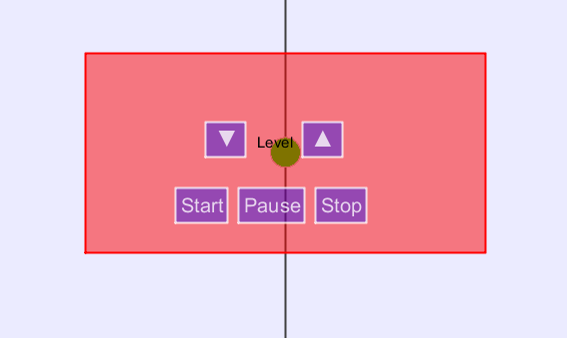
\includegraphics{../img/pong.png}
\end{center}

\end{multicols}

